\documentclass[11pt]{article}

\addtolength{\oddsidemargin}{-.875in}
	\addtolength{\evensidemargin}{-.875in}
	\addtolength{\textwidth}{1.75in}

	\addtolength{\topmargin}{-.875in}
	\addtolength{\textheight}{1.75in}


\usepackage{fancyhdr}
\usepackage{graphicx}
\usepackage{amsmath}
\usepackage{amsfonts}
\usepackage{amssymb}
\usepackage{float}
\usepackage{tikz}
 

\begin{document}


\begin{center}

 \textbf{Determining Genetic Network Dynamics Given its Logical Topology}\\
Andira Putri\\
Math 4991: Project One\\
Department of Mathematics and Statistics, Georgia State University \\

\end{center}

\textbf{I. Introduction}\\

Proteins are important molecules performing a variety of tasks. Amino acids, which are guided by a genetic code embedded in DNA, bind together to construct these proteins. Jacques Monod and François Jacob further investigated protein biosynthesis, and they discovered that an entire genetic network is responsible for protein expression. The genetic network consists of regulatory proteins called transcription factors that impact the synthesis of other proteins through either an activation or inhibition relationship. In activation, the presence of a transcription factor initiates the production of a protein. Oppositely, a protein can repress synthesis of another through inhibition. To understand activation and inhibition in a mathematical sense, they are modeled using sigmoidal Hill functions defined below in Equations 1 and 2 and shown in Figure 1:

\[ f(x)=\frac{x^n}{\theta ^n + x^n} \quad \textbf{(1)} \ \ \textrm{and}
\ \ g(x)=\frac{\theta^n}{\theta ^n + x^n} \quad \textbf{(2)} \]

\begin{figure}[h]
\centering
\includegraphics[scale=0.5]{figure1}
\caption{\textbf{Activation (left) and inhibition (right) modeled by Hill functions.} Following from Equations 1 and 2,$\theta$ is a threshold value in which the function equals 0.5. $n$ is known as the Hill coefficient that represents the maximum slope of the function. In the graphs above, larger n values result in steeper slopes. $x$ is the amount of protein present in the system. The Hill functions are bounded from 0 to 1, and $\theta$ is set to 0.5 in our graphs.}
\end{figure}

Monod and Jacob also suggested that these genetic networks may be represented using a logical (Boolean) circuit. Essentially, if a protein is expressed at a concentration above a critical threshold, it is represented as “1.” Otherwise, a protein is represented as “0,” meaning there is very little or none of it in the system. The “1” and “0,” known as truth values, are the fundamental outputs of a logical circuit, and they can change with each time step. In Dynamics in Genetic Networks by Roderick Edwards and Leon Glass, the logical circuit framework is exploited to answer the following question: \textit{given the logical structure of a biological system, is it possible to determine the dynamics of the network?}

\begin{center}
\end{center}
\textbf{II. Results}\\

The problem is approached using methods of differential equations, dynamical systems, and numerical analysis. To begin, we consider the biological foundations of the genetic network. Because activation and inhibition relationships impact the amount of protein created, we use the Hill functions in Equations 1 and 2 to model production. All proteins will naturally unbind or deplete through random processes. For simplification, we assume that a protein degrades at a constant rate. To piece together production and degradation, we use an intuitive differential equation:
\begin{center}
\textit{Rate of change of x = production of x - degradation of x} \textbf{(3)}.
\end{center}

An example of a genetic network with two inhibiting nodes is shown below in Figure 2.  

\begin{figure}[h]
\centering
\includegraphics[scale=0.4]{figure2}
\caption{\textbf{Two-gene mutually-inhibiting network.}}
\end{figure}

For the simple two-gene mutually-inhibiting network, we use Equation 3 as a template for the following system of ordinary differential equations, with A and B as variables:

\[ \frac{dA}{dt}= 0 = g(B) = A \quad \textbf{(4)} \ \ \textrm{and}
\ \ \frac{dB}{dt}= 0 = g(A) = B \quad \textbf{(5)} \]

Notice that “-x” represents the natural degradation, and “g(x)” represents the inhibition relationship. To investigate the dynamics of the system, we find the curves in which $dA/dt$ and $dB/dt$ both equal 0; they are called \textit{nullclines} \textbf{[2]}. The nullclines for our system are drawn below in Figure 3, and the trajectories are shown to give an overall phase portrait. We observe that there is a saddle point at A = B = 0.5, so we define that point as the critical threshold. We derive a state transition table which offers a simplified visual of the phase portrait given the logical structure of the network, shown below in Figure 3. Because of the dynamical behavior of this system, we define the network as a “toggle switch.”

\begin{figure}[H]
\centering
\includegraphics[scale=0.4]{figure3}
\caption{\textbf{Phase portrait (left) and the resulting state transition diagram (right) of two-gene mutually-inhibiting network.} The nullclines intersect at (1,0), (0,1), and (0.5,0.5) to give three fixed points. The points at (1,0) and (0,1) are stable nodes, so trajectories will go towards the corresponding logic state, 10 and 01, respectively. (0.5,0.5) is an unstable saddle point, so trajectories will diverge from this point. (0.5,0.5) is also known as the threshold point. The state transition diagram on the right is a simplified version of the phase portrait, following the same trajectories and representing the logical foundation of the genetic network.}
\end{figure}

Now, consider a three-gene mutually-inhibiting circuit (namely, a repressilator), depicted in Figure 4 and modeled by: 

\begin{center}
\( \frac{dA}{dt} = g(C) - A \)  \quad \textbf{(6)} \linebreak
\( \frac{dB}{dt} = g(A) - B \)  \quad \textbf{(7)} \linebreak
\( \frac{dC}{dt} = g(B) - C \)  \quad \textbf{(8)}
\end{center}

\begin{figure}[H]
\centering
\includegraphics[scale=0.4]{figure4}
\caption{\textbf{The repressilator.}}
\end{figure}

This system offers more complications. Suppose protein A inhibits B, protein B inhibits C, and protein C inhibits A. If there is a large concentration of A, less of B is produced. Due to the low concentration of B, more of C is created because not enough B is available to repress C. Then, the high levels of C will repress A’s creation and lower A’s amount in the system. The cycle continues, and this results in an oscillation between the three proteins’ concentrations, shown in Figure 5. Recall that in the two-gene network, we end in one of two states: “01”  or “10.” However, in our three-gene network, the states always fluctuate since all proteins oscillate from high to low expressions. We call this phenomenon “frustration,” and the everlasting need to modify states denotes system instability. The instability is represented in the state transition diagram, shown in Figure 5.

\begin{figure}[H]
\centering
\includegraphics[scale=0.4]{figure5}
\caption{\textbf{Oscillations in the concentrations of A, B, and C (left) and the corresponding state transition diagram (right).} The state transition diagram is based on a logical rule which results in a truth table given in Figure 6. }
\end{figure}

Notice that the repressilator state transition diagram was not based on nullcline phase portraits, like the two-gene mutually-inhibited network. Instead of drawing nullclines in three dimensions, we use truth tables to define the dynamics, using the following equation:

\begin{center}
$X_i(t+1) = F_i(X_{i_1}(t), X_{i_2}(t),...,X_{i_K}(t));  i = 1, 2,...,N $ \quad \textbf{(9)}
\end{center}

Equation 9 describes the Boolean switching network, and the resulting $X(t+1)$ is either “1” or “0.” $x_1, x_2,..,x_K$ are truth values for a total of K previous time steps that will determine the state in the next time step, given the relationships between proteins (activation or repression) in the genetic network. Thus, we obtain a truth table, shown in Figure 6, which our state transition diagram is based on.

\begin{figure}[H]
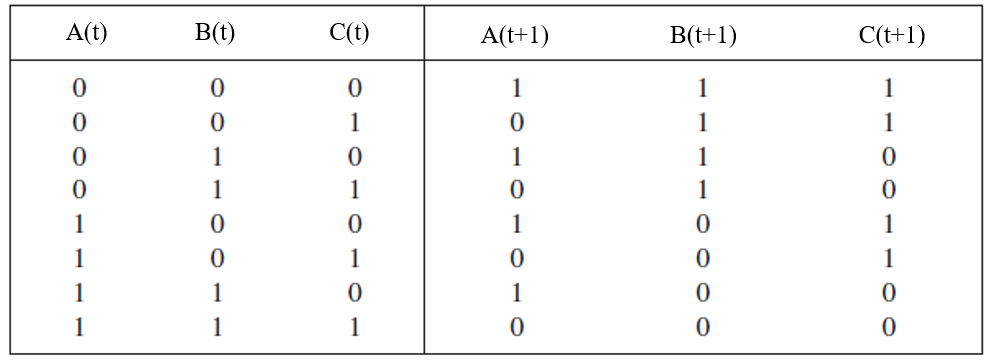
\includegraphics[scale=0.5]{Table1}
\centering
\caption{\textbf{Truth table defining the paths of the state transition diagram for the repressilator.}}
\end{figure}

Of course, we may extend these methods beyond two and three gene networks. To derive a model for a network of N genes, we must take advantage of truth values. For simplification, we define 0 to be the critical threshold concentration. Then, we combine our variables and their truth values to formulate a rule based on time steps:

\begin{center}
$X_i(t) = 0$ if $x_i(t) < 0$; otherwise, $X_i(t) = 1$ \quad \textbf{(10)}
\end{center}

Applying the template in Equation 3, we get:

\begin{center}
\( \frac{dx}{dt}\) $= f_i(X_{i_1}(t), X_{i_2}(t),...,X_{i_K}(t)) -  x;  i = 1, 2,...,N $ \quad \textbf{(11)}
\end{center}

where the production term in Equation 10 takes the truth value defined by Equation 9. Creating a phase portrait based on nullclines is a difficult task in this scenario since we would be solving a system of N differential equations, so we use numerical integration. To begin, we must understand the network topology and section the space into orthants. To illustrate, the two-gene network is divided into the “00,” “01,” “10,” and “11” orthants. Next, we acknowledge that all orthants will have trajectories leading to a fixed point, or focal point. If a trajectory from one orthant goes towards a fixed point in different orthant, we assume that protein concentration crosses the threshold, and the system projects to a focal point in the new section. The template given in Equation 3, used in Equation 11, is mathematically simple, so we numerically integrate 11 to obtain the general solution, shown by Equation 12 \textbf{[1,4]}. Essentially, we are finding the set of times in which the concentration of protein is 0 using the following for $t_j<t$:

\begin{center}
$x_i(t) = x_i(t_j)(e^(t_j-t)) + f_i(X_{i_1}(t), X_{i_2}(t),...,X_{i_K}(t))(1-(e^(t_j-t)))$ \quad \textbf{(12)}
\end{center}

However, if concentration is never 0, meaning the concentration never crosses the threshold, the trajectory will go towards a steady state in its respective orthant. The process is then iterated. (The paper goes more into numerical methods using Hamming distance, but I was not able to find resources to understand it.) To construct the N-cube, we draw a directed edge that represents the trajectory flow between orthants, where the edges are the shortest path between vertices $t$ and $t+1$. This information is given by Equation 12; we employ the set of times when the threshold is crossed (concentration is 0) because that causes the transition between truth values.  Once all edges are complete, we have an N-cube showing the system dynamics given the logical structure of a genetic network, which answers our big question.

I will not be going over the analysis methods for the N-cube, which goes into chaotic dynamics (did not understand and was not important to the goal of the paper). 

\begin{center}
\end{center}
\textbf{III. Comments}\\

In the paper, the authors did not use any networks with solely activation relationships, and I understood the reason why. Consider the two-gene mutually-activating network in Figure 7. Due to the behavior of the network, the concentrations of both A and B will continuously increase. In Calculus I terms, the limit of both proteins’ concentrations as time approaches infinity...is infinity. Therefore, a network with just activation is incredibly unstable. Of course, this holds for networks of three or more genes as well. Despite this fact, it would have been useful to see genetic networks with both activation and inhibition, as not all biological systems are mutually-inhibiting. I thought about doing this with my biofilm project, but a ten-dimensional cube with chaotic dynamics seems too far out of my reach.

\begin{figure}[h]
\centering
\includegraphics[scale=0.4]{figure6}
\caption{\textbf{Two-gene mutually-activating network.}}
\end{figure}

In population biology, you could think of the two-gene mutually-inhibiting network as almost similar to the Lotka-Volterra predator-prey model. The only major differences are that the interaction term is not modeled by a Hill function \textbf{[2]}, which will impact the nullclines and therefore the phase portrait, and prey do not necessarily inhibit predators. However, the more predators you have, the less prey there will be, which represents inhibition. 

Regarding the pedagogical structure of the paper, I found the organization completely out of order. The authors placed the state transition diagram in Figure 3 two pages before the phase portrait. They solely based the state transition diagram on a (personally) misleading truth table. Also, the paper did not introduce basic information about system stability (nullclines, eigenvalues, fixed points, etc.) and meaning of results until almost the END of the article. I did not explain this part of the article in the results section because it was redundant at that point.


  \begin{thebibliography}{1}

  \bibitem{1} Richard L. Burden and Douglas J. Faires, {\em Numerical Analysis,
  Cengage Learning.}  2016.

  \bibitem{2}  Leah Edelstein-Keshet {\em Mathematical models in biology, SIAM} 2005:
  Random House, N.Y.

  \bibitem{3} Roderick Edwards and Leon Glass {\em Dynamics in Genetic Networks} 2014: American Mathematical Monthly
  Relations.

  \bibitem{4} {\em Numerical Methods for Differential Equations} 1986: Olin College.

  \end{thebibliography}
\end{document}


